\subsection{Logical View}

\copied{Logical view : The logical view is concerned with the functionality that the system provides to end-users. UML Diagrams used to represent the logical view include Class diagram, Communication diagram, Sequence diagram.[2]}
{from wikipedia\\\url{https://en.wikipedia.org/wiki/4\%2B1_architectural_view_model}}

Desision: Push model reduces the server load. No requests so no high load. No data management, no security management. No DOS.
Downside: Data will be received that was not requested, even if not interested. 

Pix4D software automatically processes terrestrial and aerial imagery acquired by light-weight drones or aircraft using its innovative technology based purely on image content. This desktop software converts your images into highly precise, timely and customizable results for a wide range of GIS and CAD applications.
\url{https://pix4d.com/}
This view shows the structural elements, key abstractions and mechanisms that are used within HPS to realize the systemics functionality. At first an overview of the components is provided. After that the main components are decomposed and desired in term of responsibilities and interfaces. In the end, the variability guide mentions parts of the software, which clarification is deferred until development/design phase.
\clearpage
\begin{figure}[hb!]
%\centering
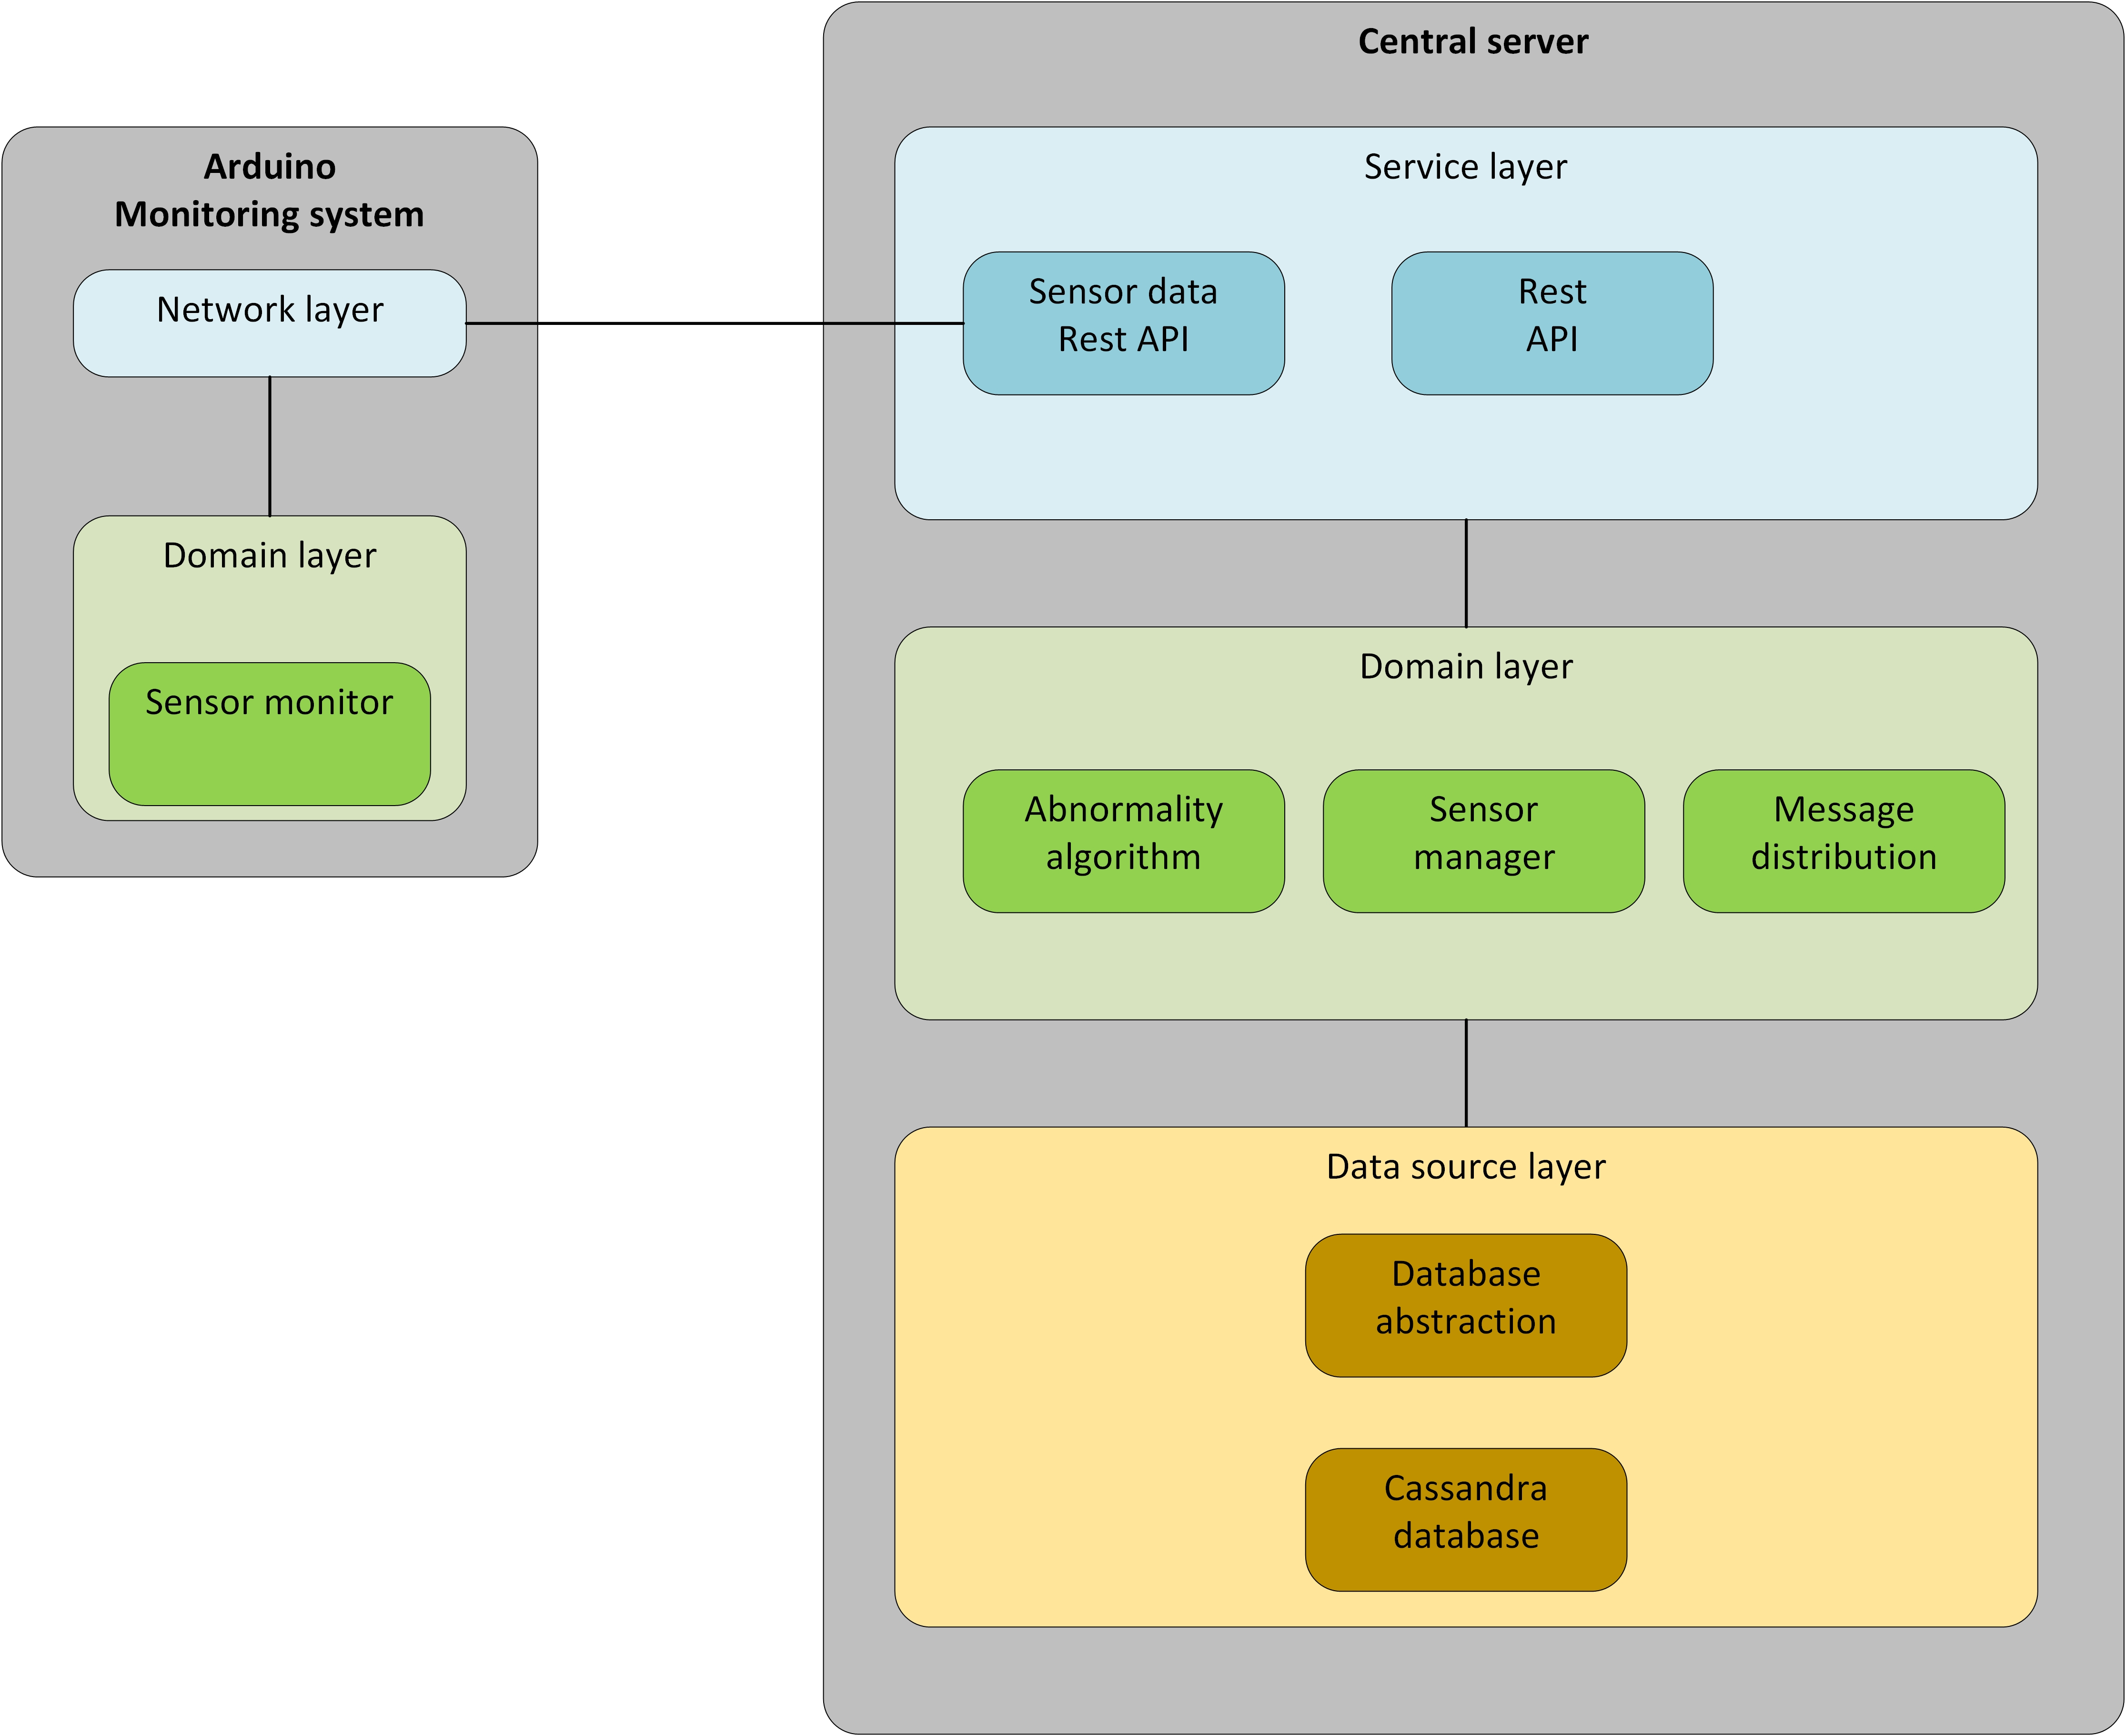
\includegraphics[keepaspectratio=true,width=0.9\textwidth]{{\viewimages/layers}.jpg}
\caption{Layers of the software}
\label{fig:layers}
\end{figure}

\clearpage
\begin{sidewaysfigure}[hb!]
%\centering
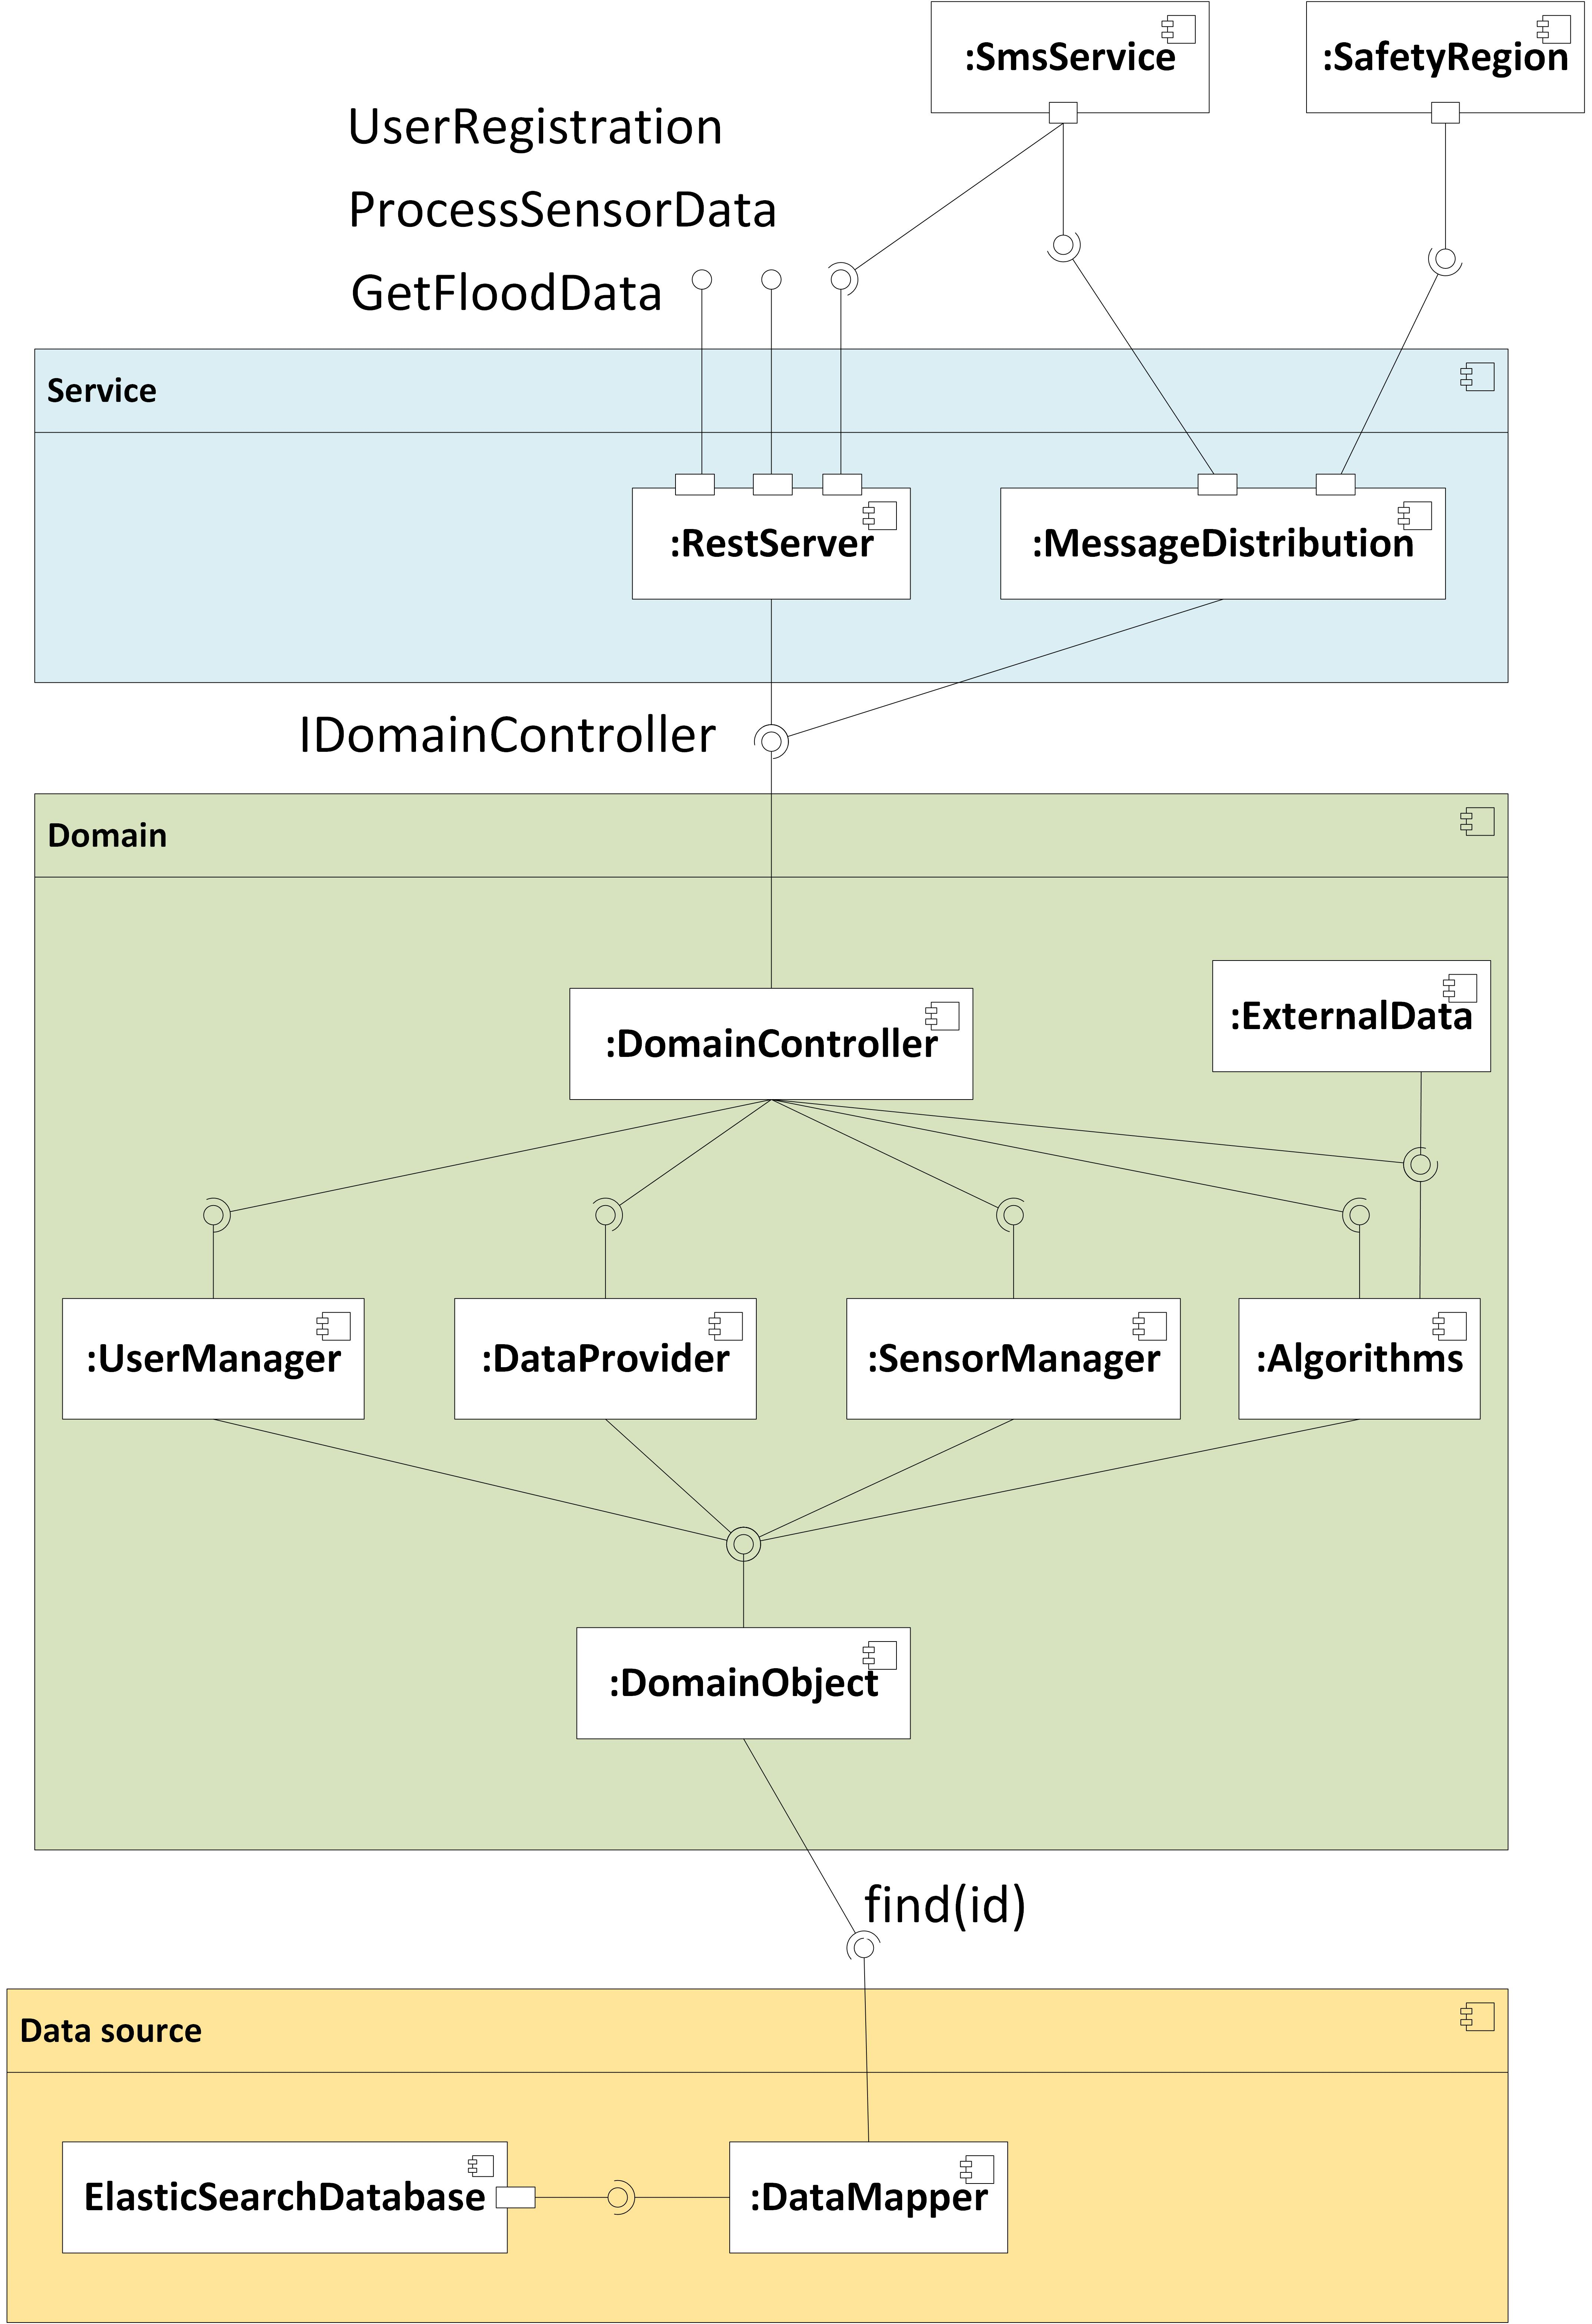
\includegraphics[keepaspectratio=true,width=0.9\textwidth]{{\viewimages/component}.jpg}
\caption{Component diagram}
\label{fig:component}
\end{sidewaysfigure}

\clearpage
\begin{figure}[h]
%\centering
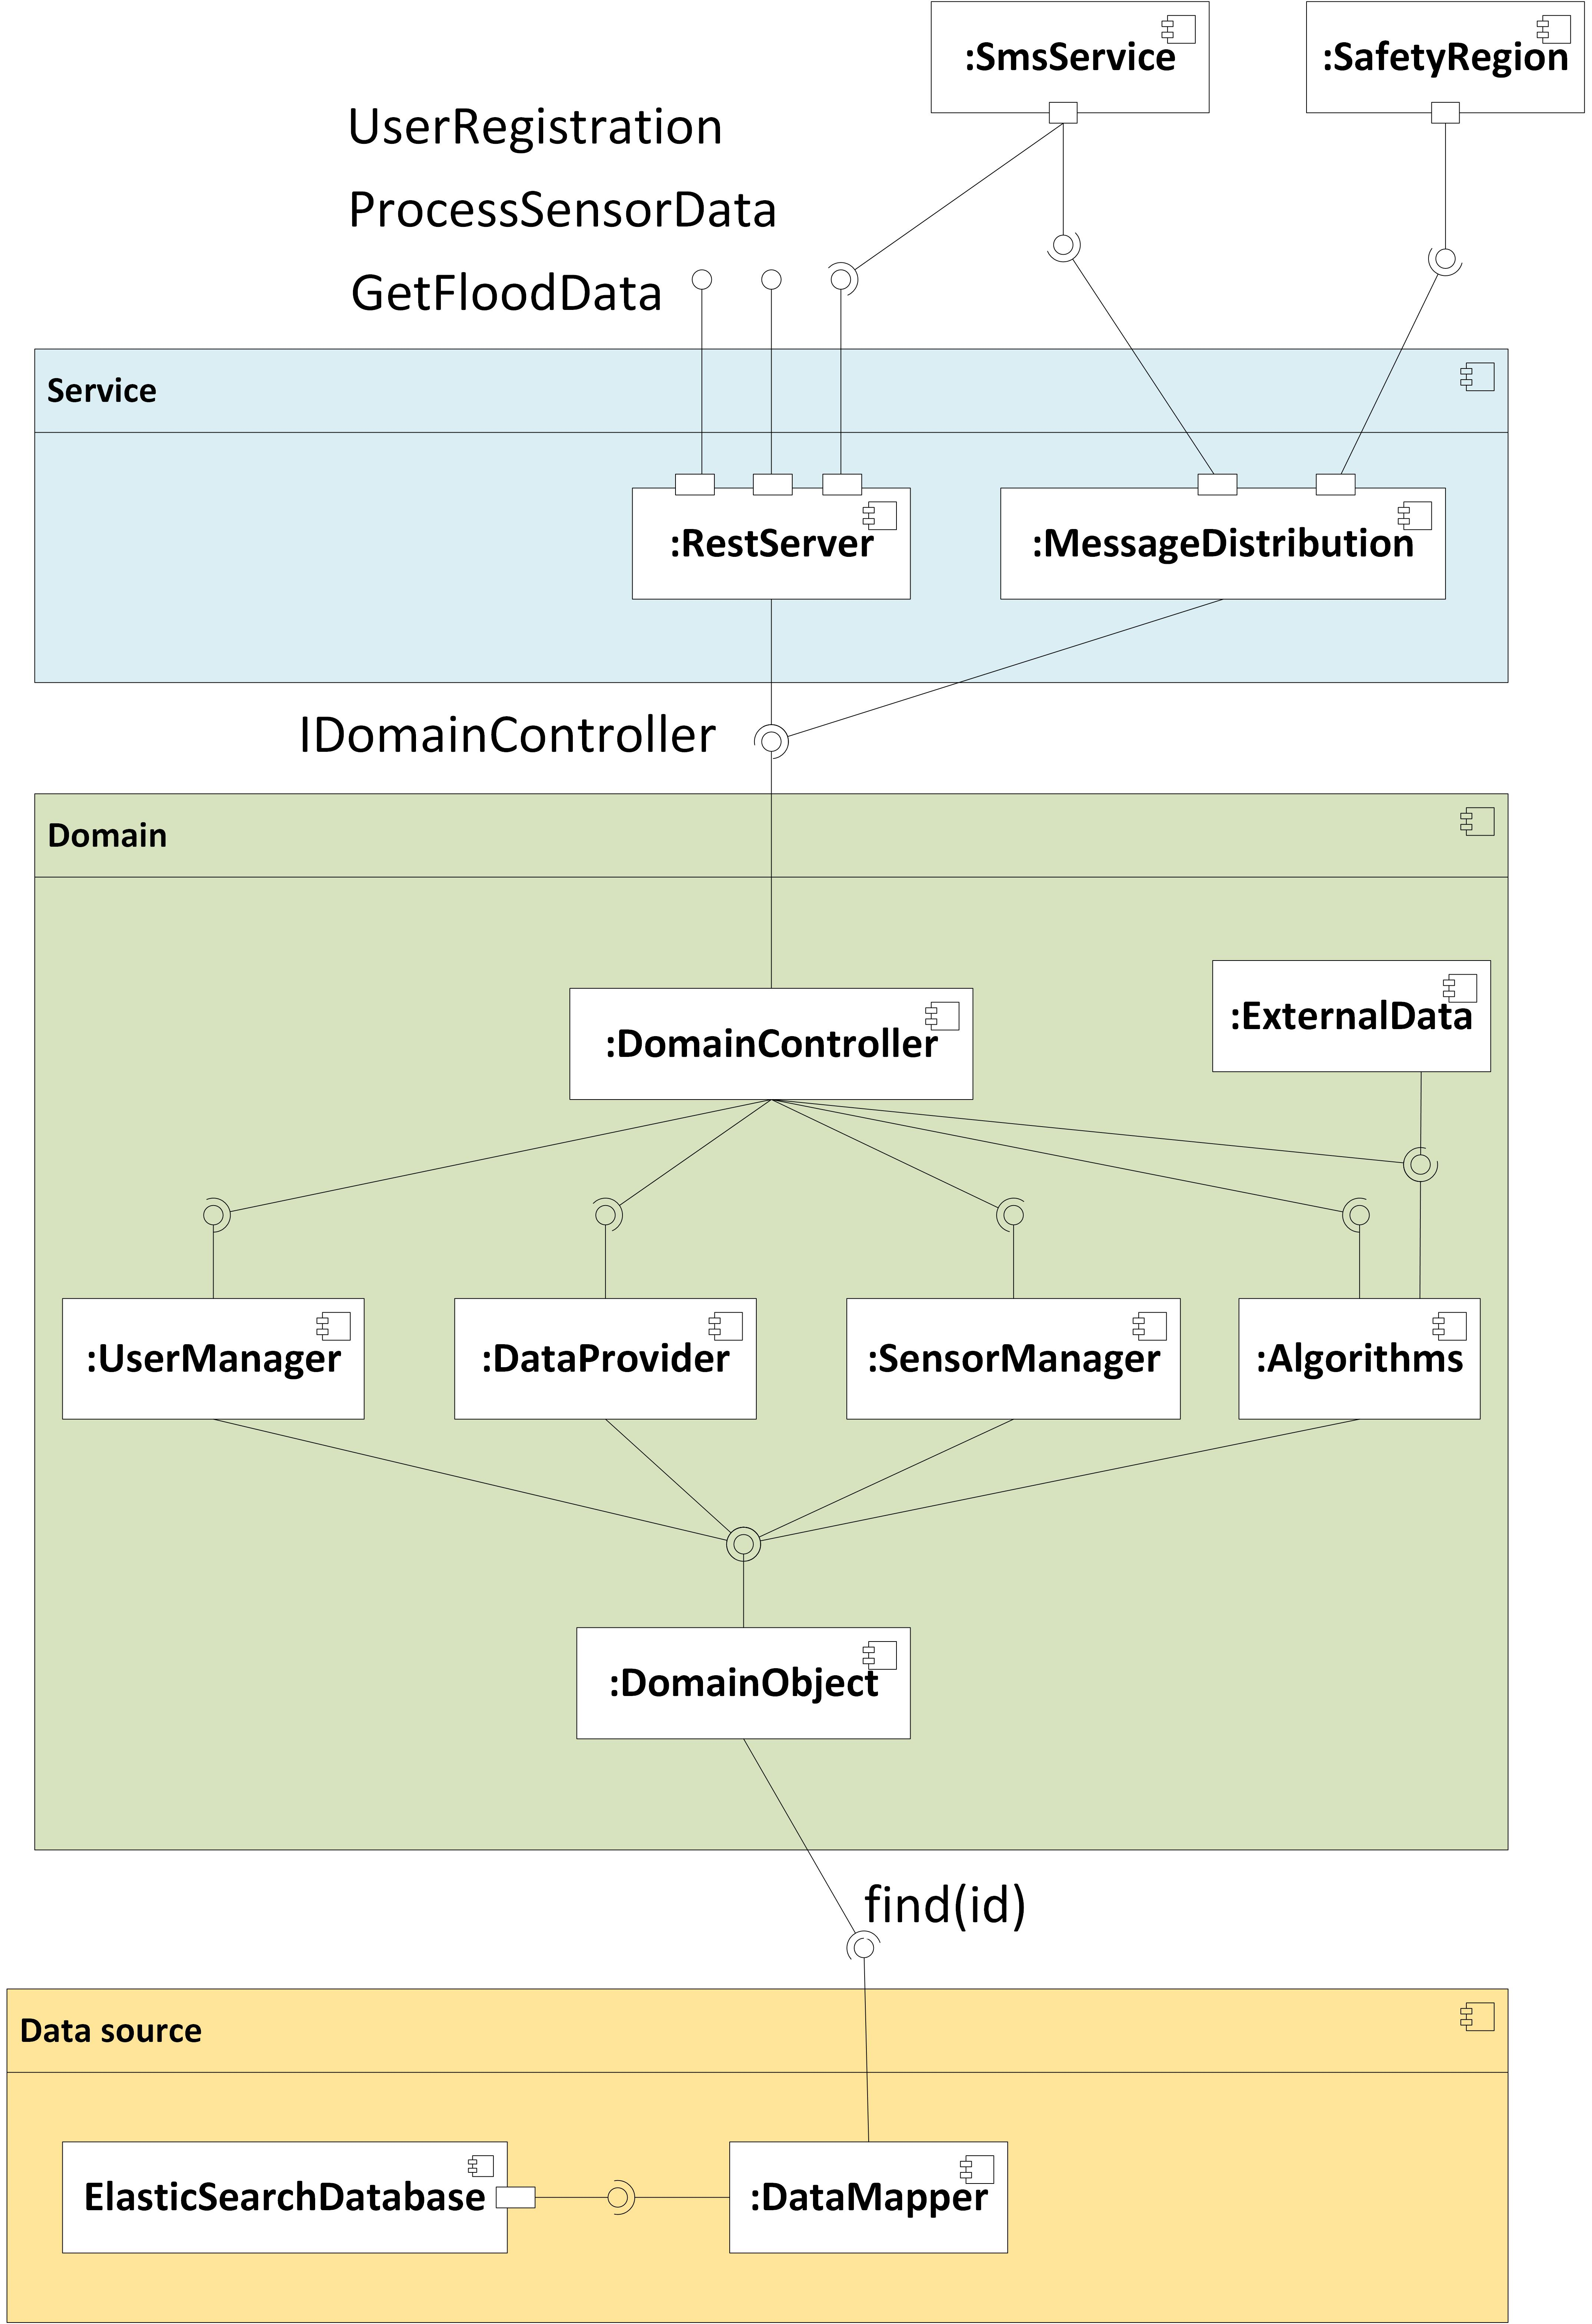
\includegraphics[keepaspectratio=true,width=0.9\textwidth]{{\viewimages/component}.jpg}
\caption{Component diagram}
\label{fig:component}
\end{figure}

\begin{figure}[hb!]
%\centering
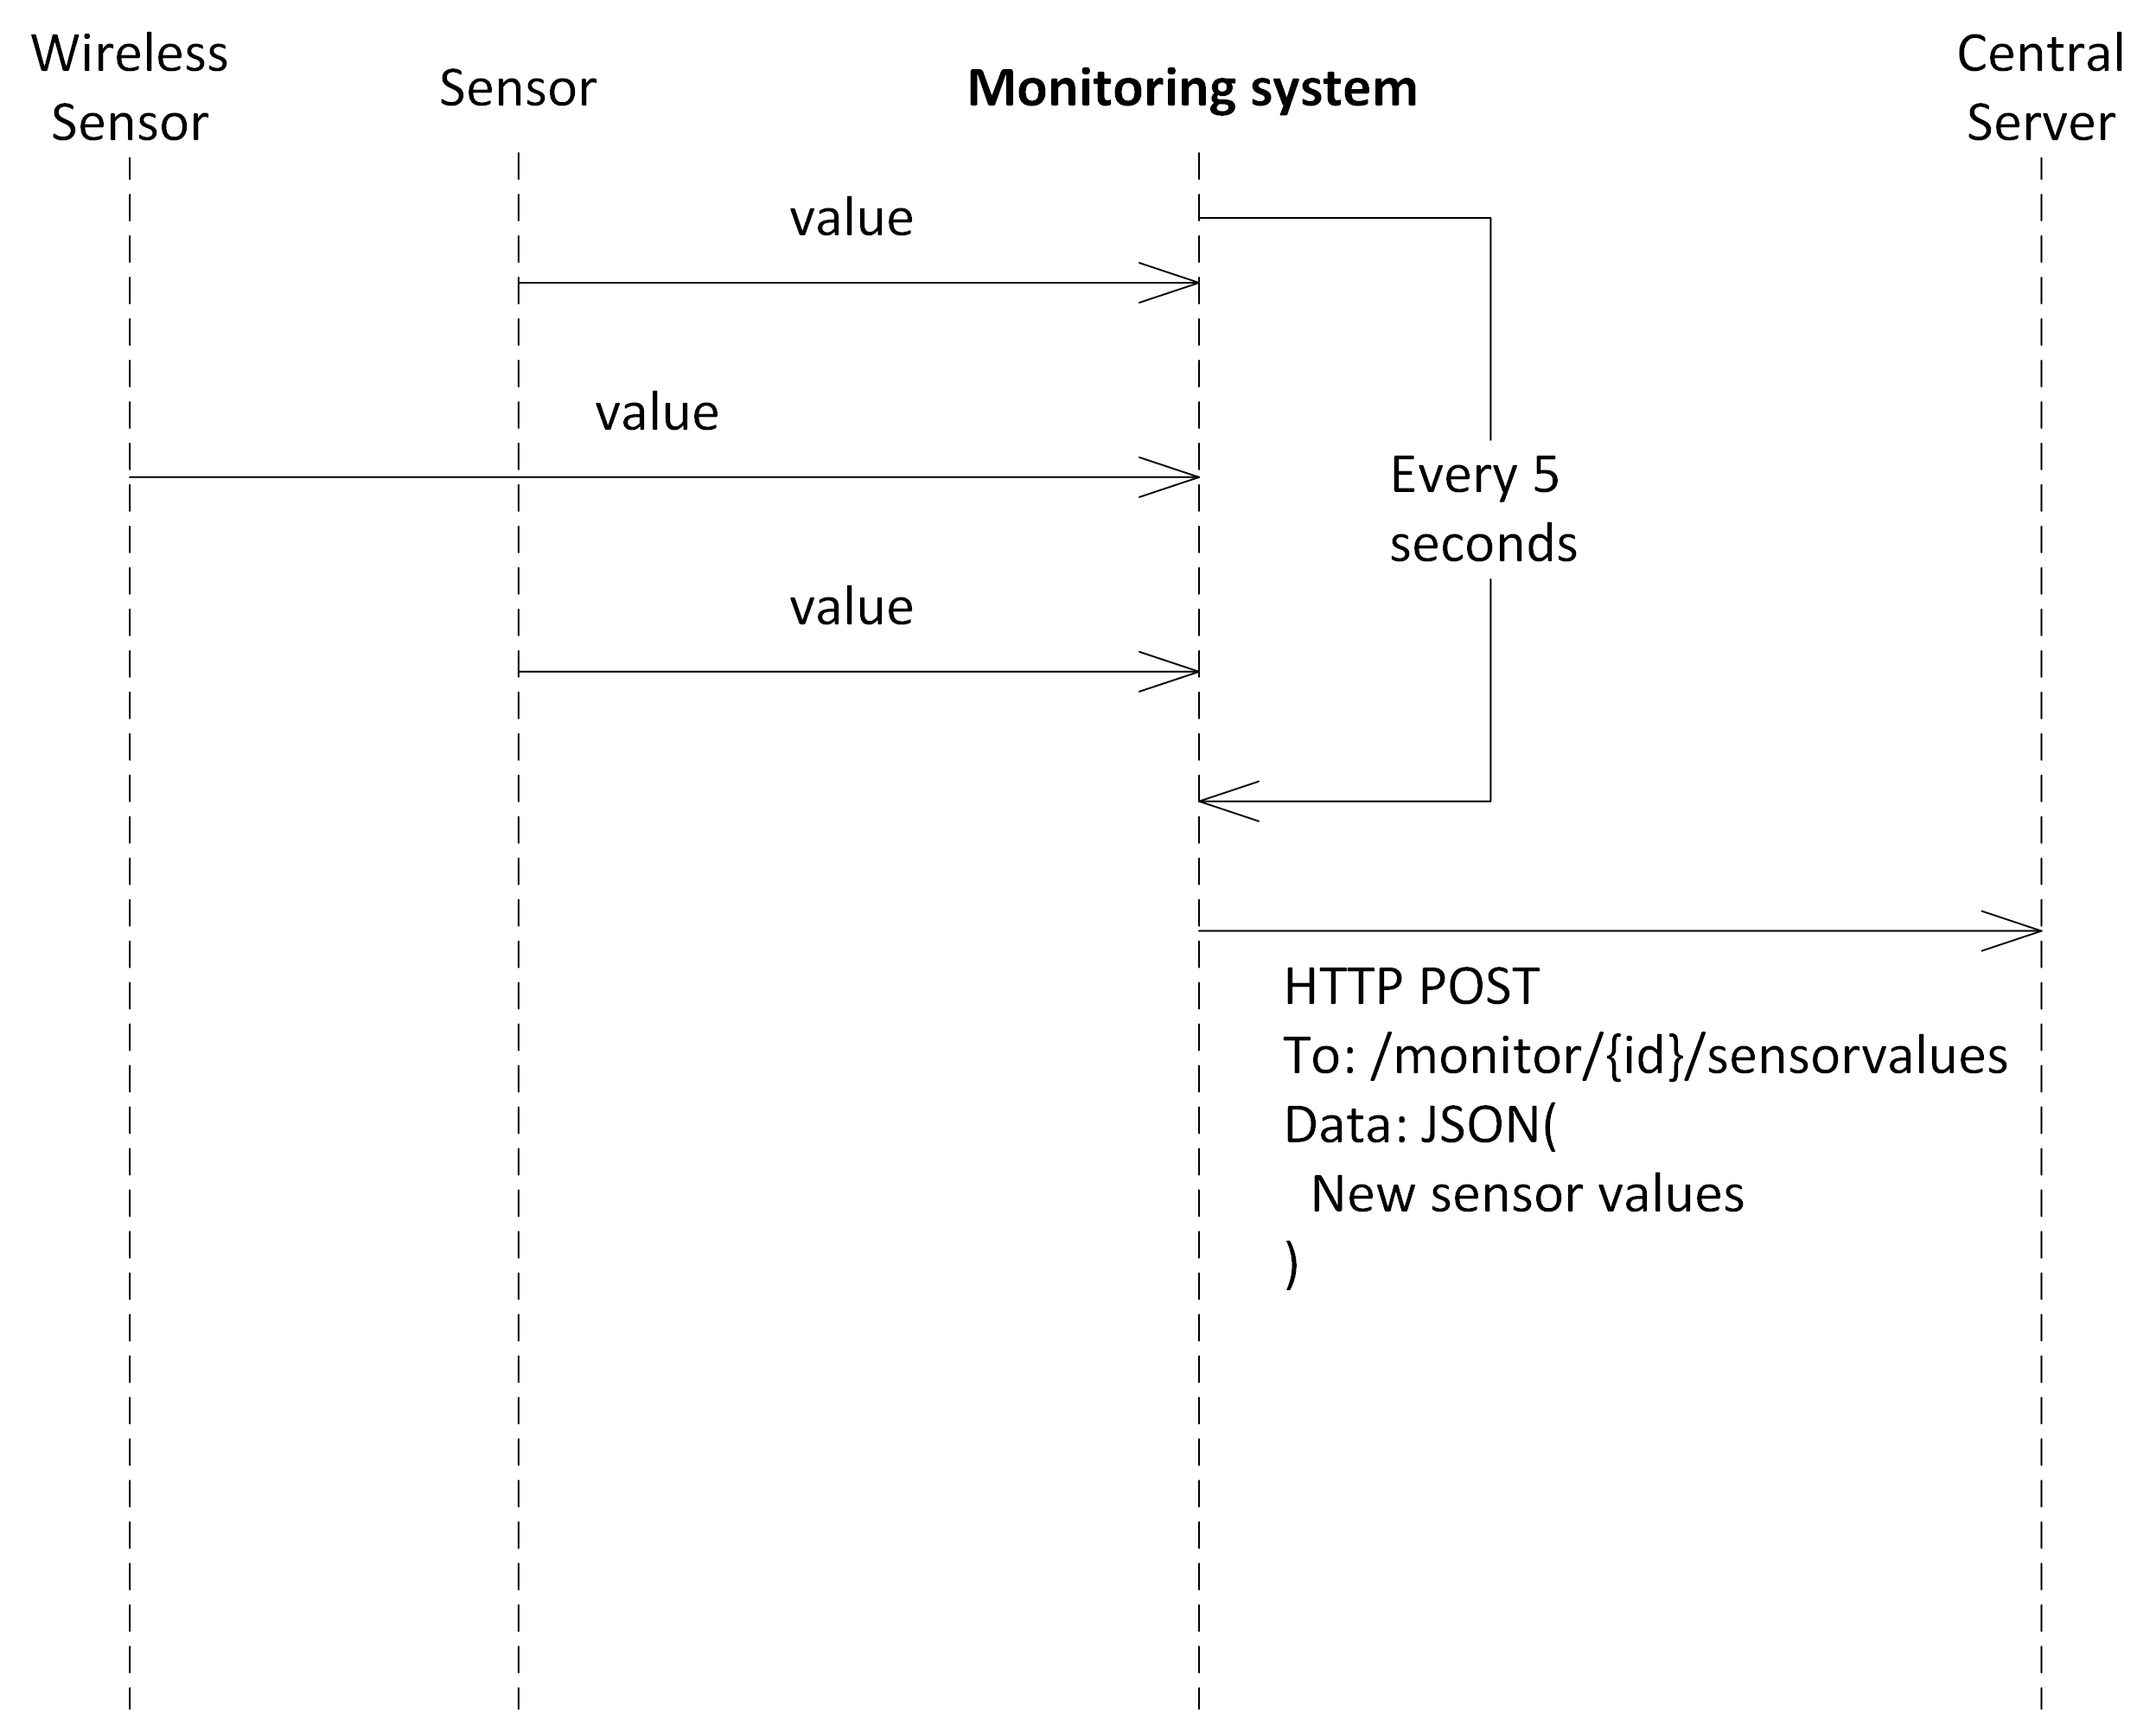
\includegraphics[keepaspectratio=true,width=0.9\textwidth]{{\viewimages/sequence1}.jpg}
\caption{Sequence diagram of the client pushing the sensor data}
\label{fig:component}
\end{figure}

\clearpage
\begin{figure}[hb!]
%\centering
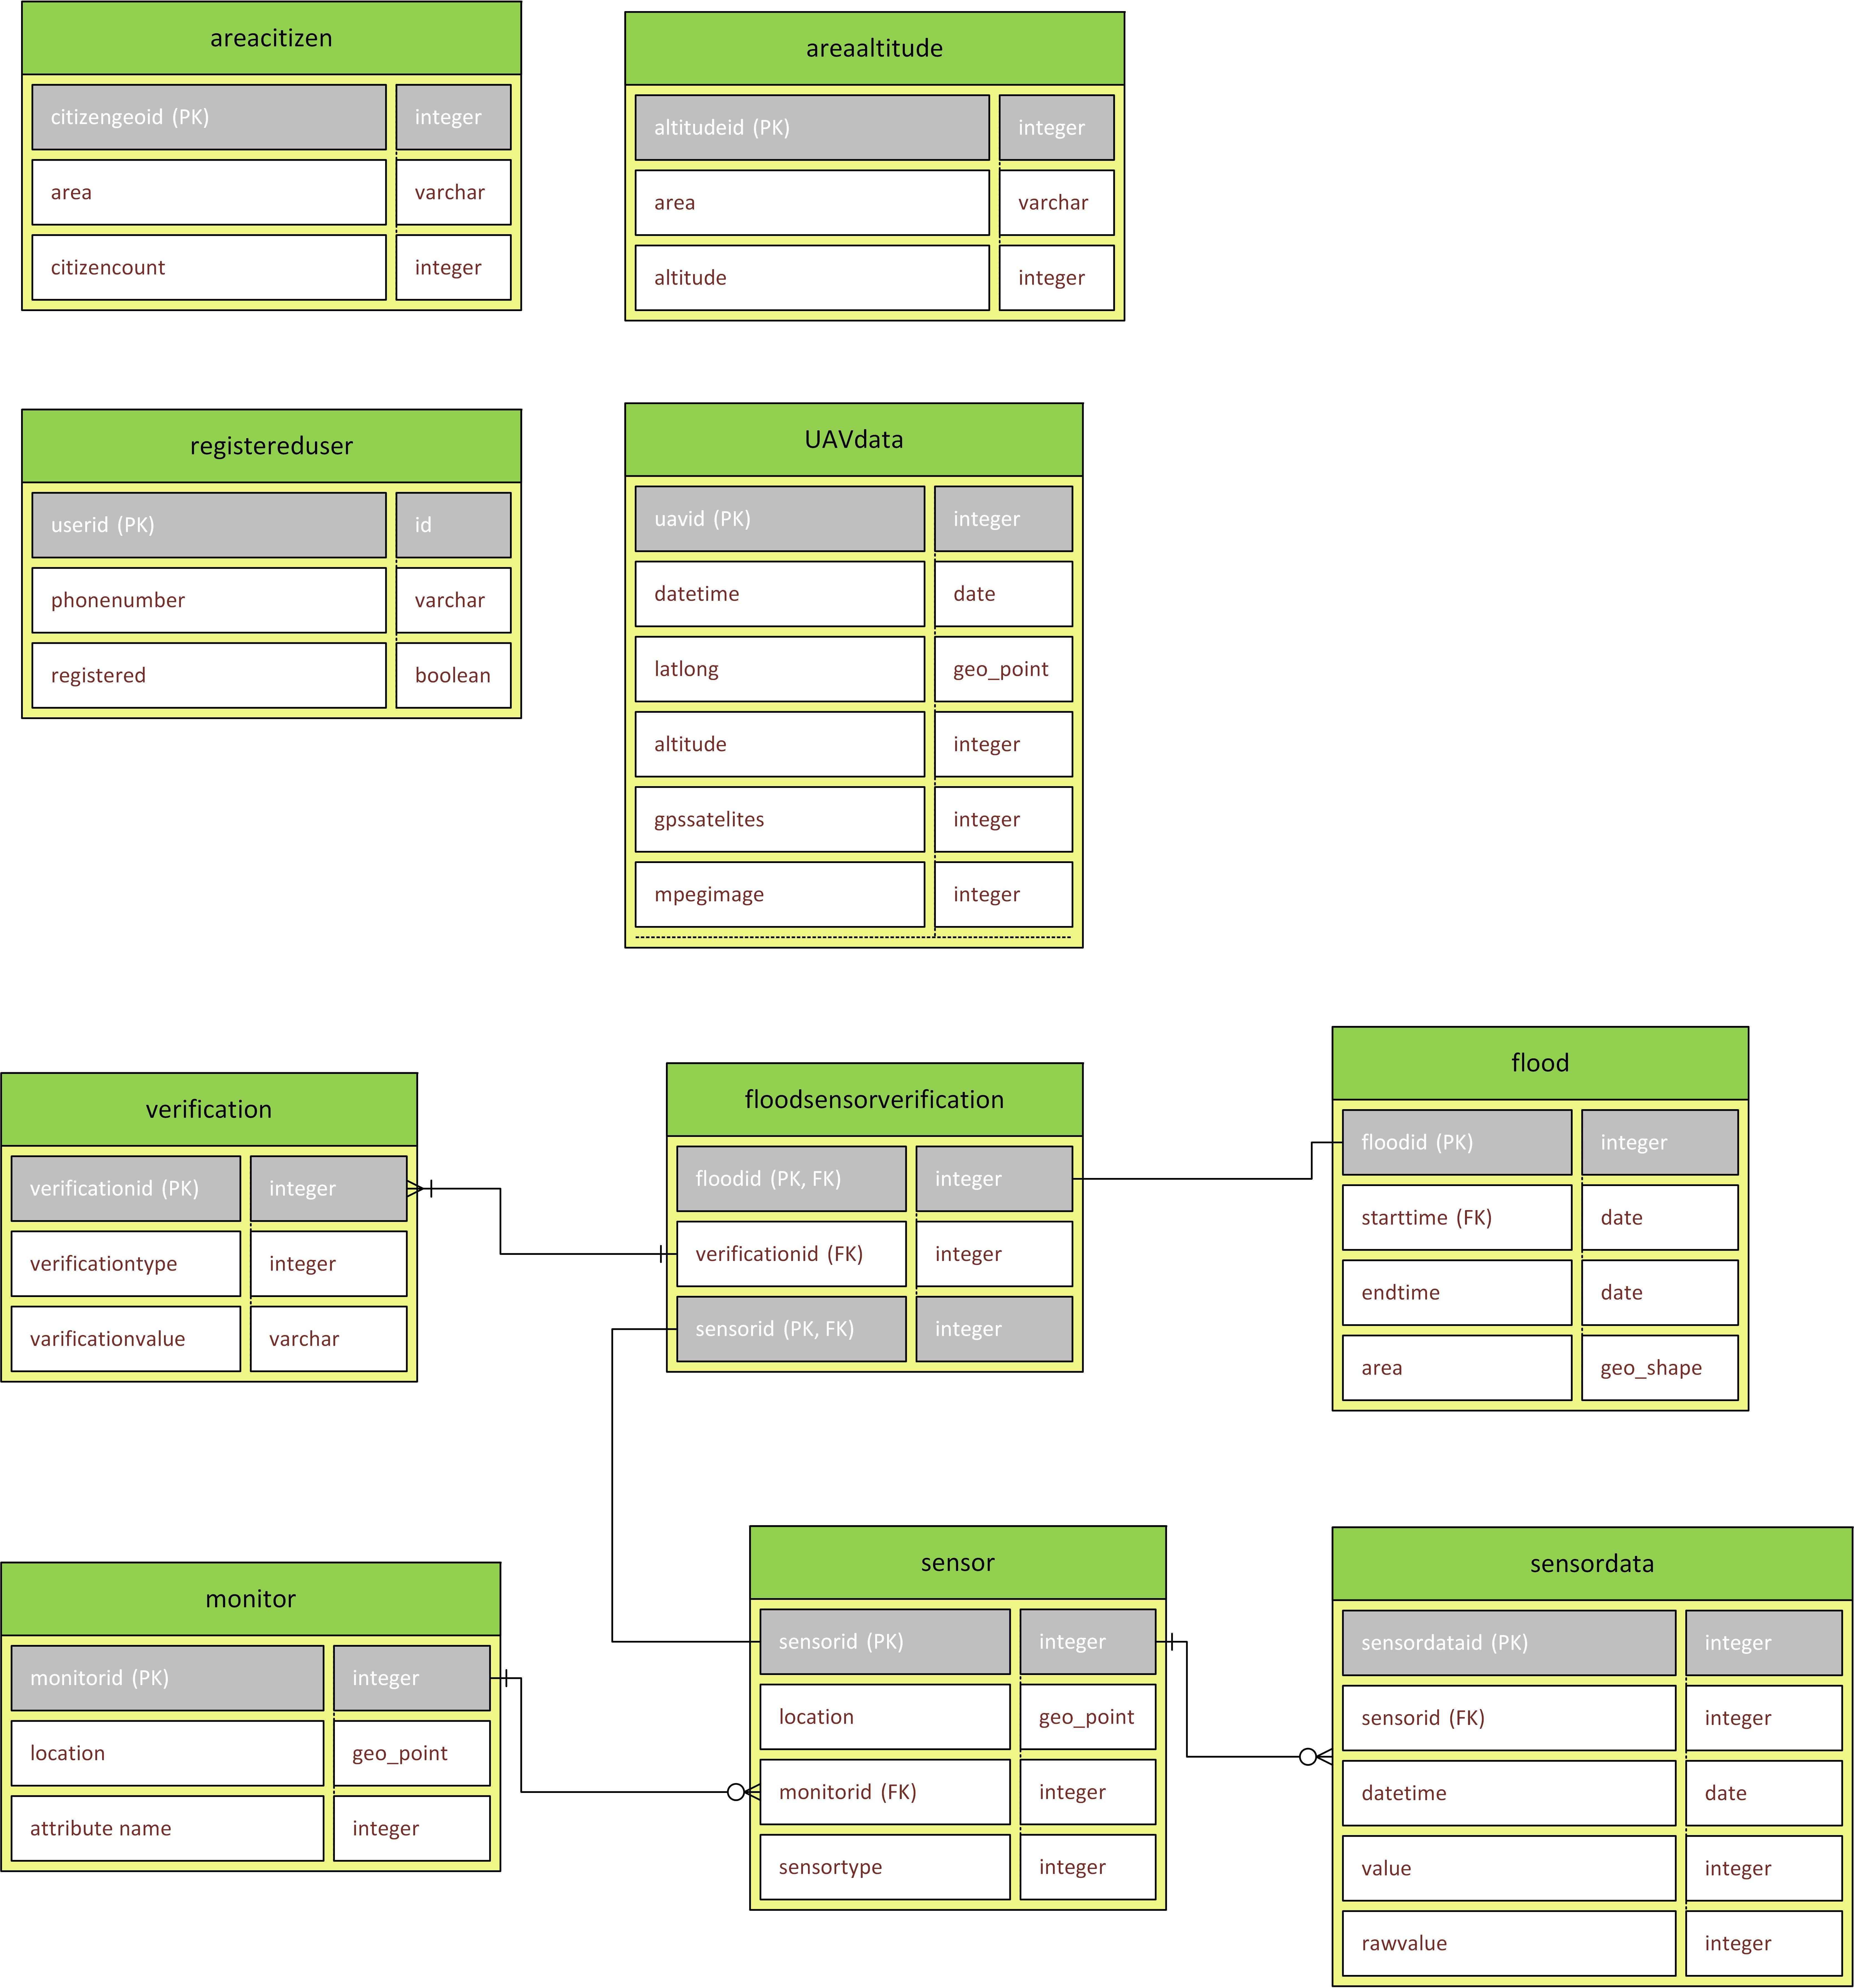
\includegraphics[keepaspectratio=true,width=0.9\textwidth]{{\viewimages/database}.jpg}
\caption{Database diagram}
\label{fig:component}
\end{figure}

\begin{framed}
	Data Mapper for the data layer.
	alternatives: table data gateway, active record, ...
\hrule
	Update monitor system firmware? Do we do this? And how do we do this?
	Do sensors have firmware and how do we update that?
\hrule
	
	In db:
	Verificationtype = uav, person of none?
\hrule

	Storing and querying geo data in cassandra using datastax in java
	http://digbigdata.com/geospatial-search-cassandra-datastax-enterprise/
	desision: maybe use an other database for this kind of data? 
	ElasticSearch seams to be popular https://www.elastic.co/
\end{framed}

